\begin{figure*}[!ht]
  \centering
  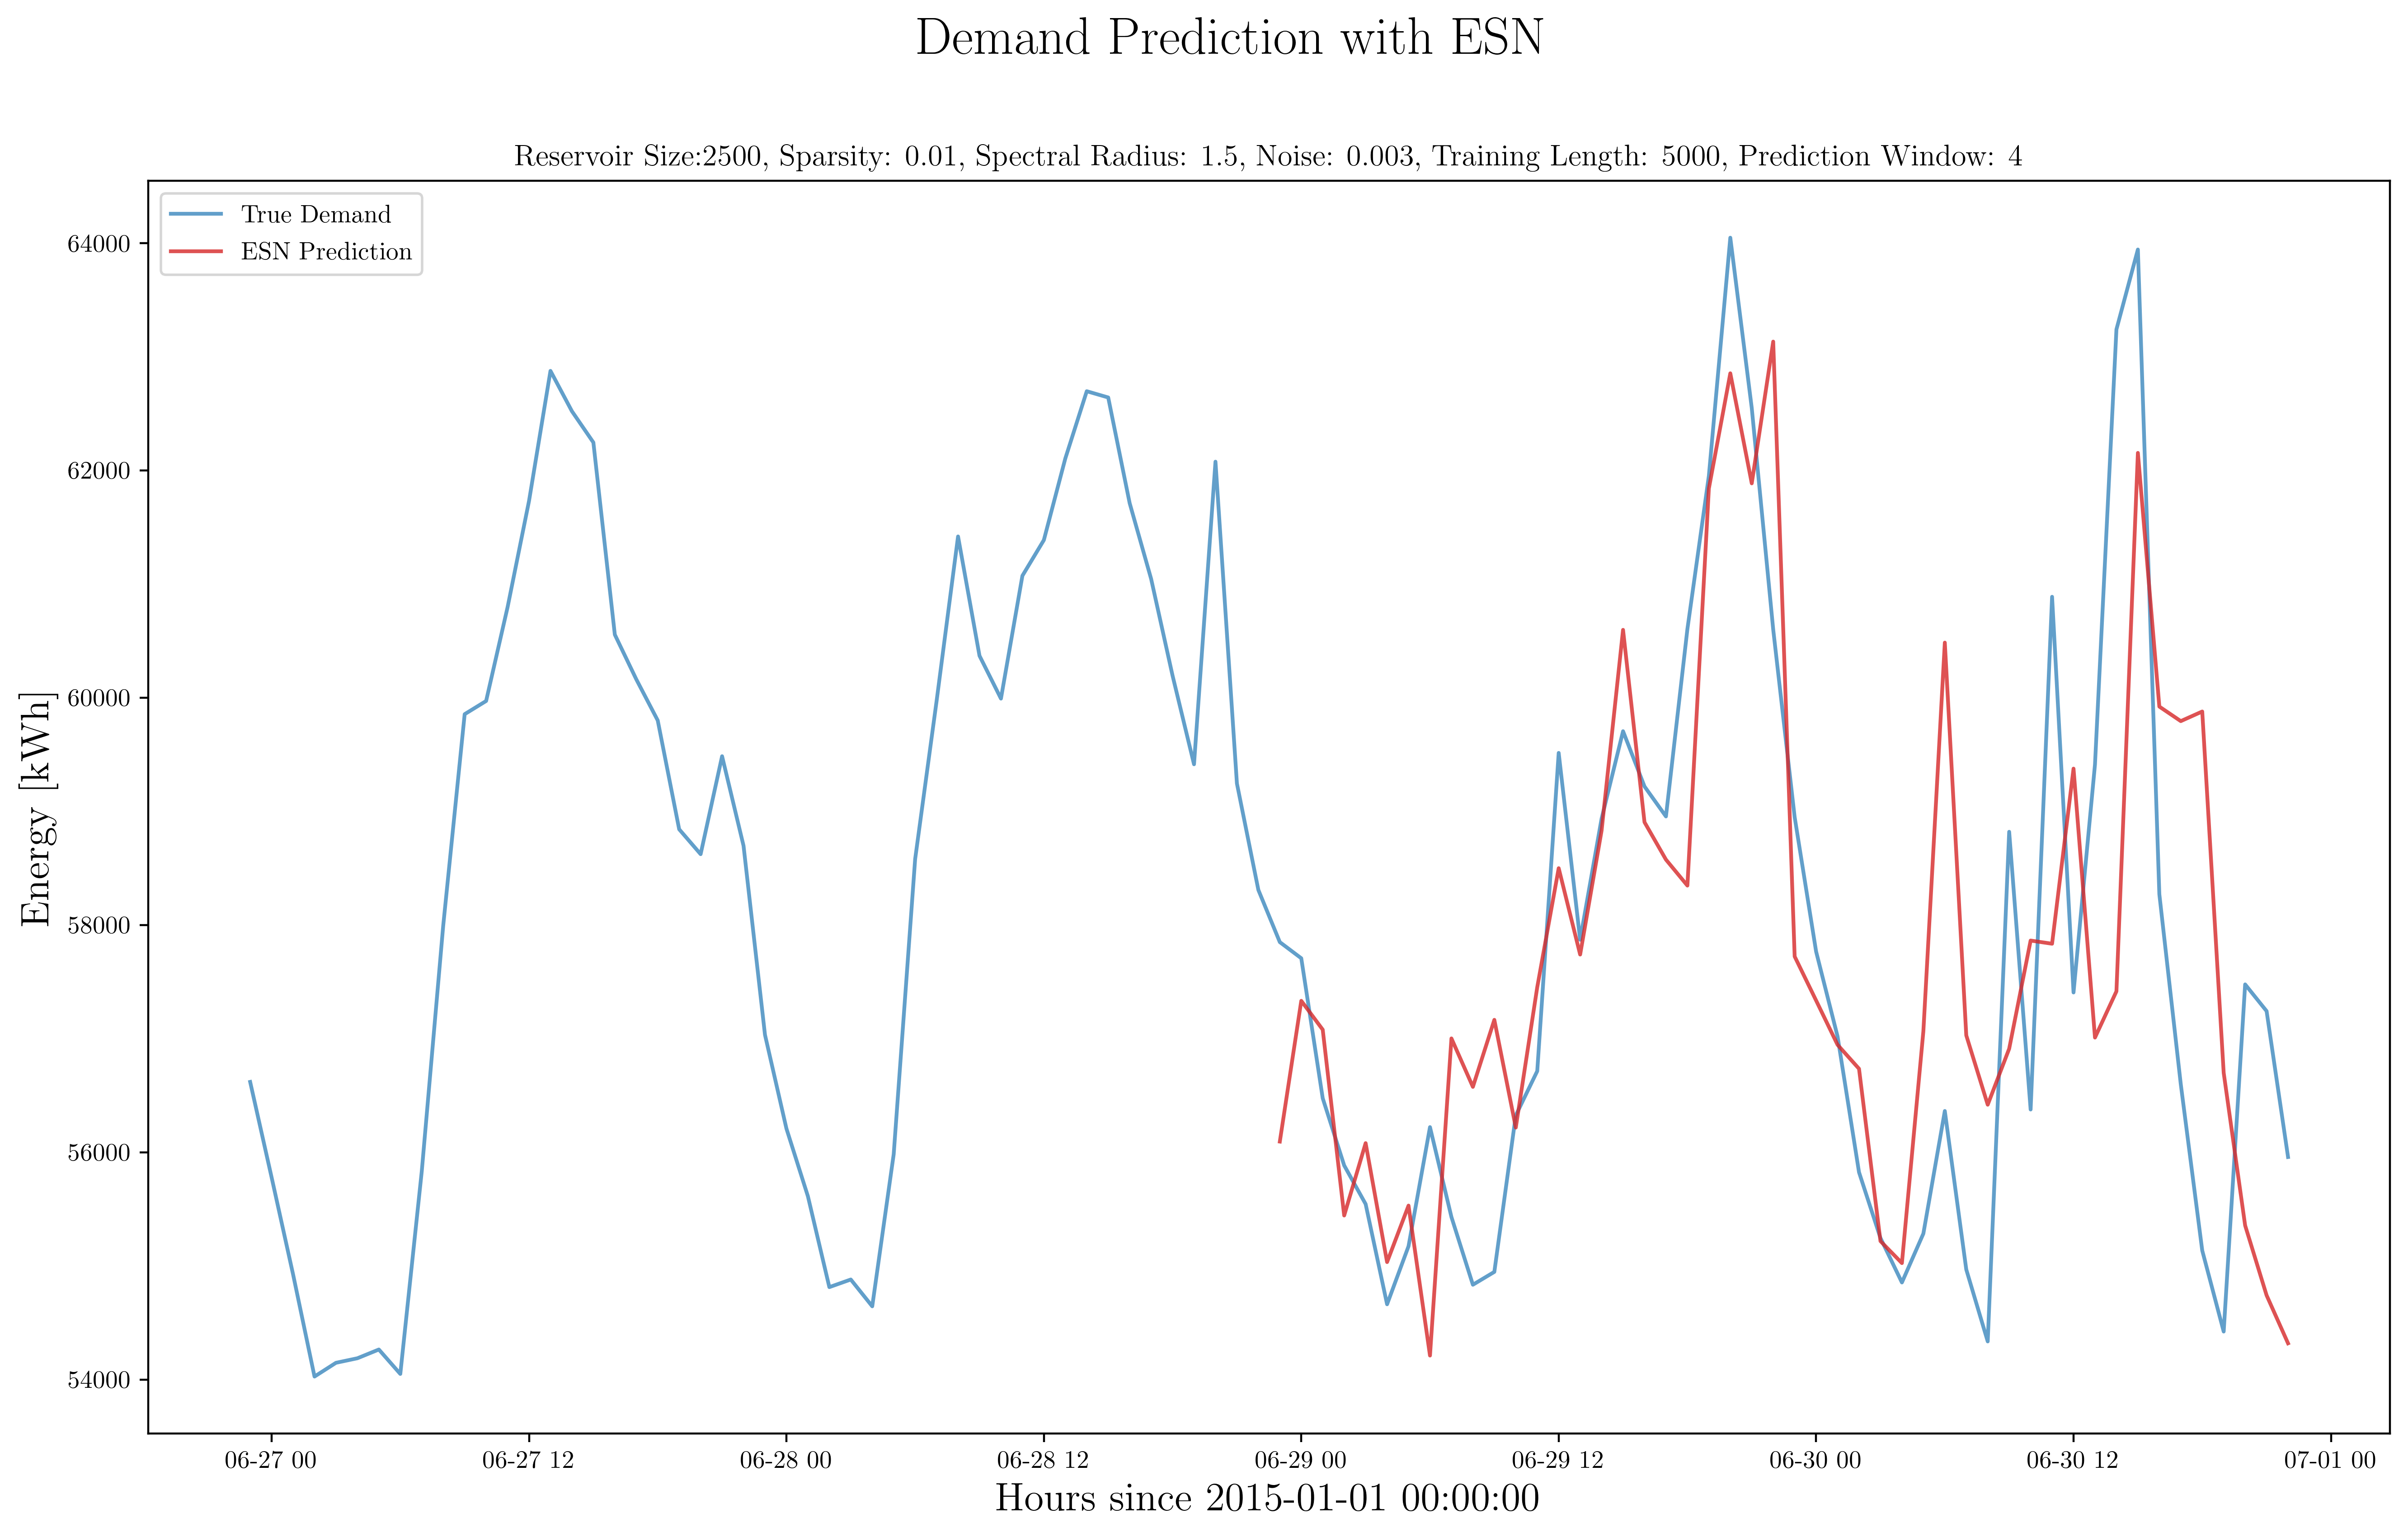
\includegraphics[width=0.8\textwidth]{04_demand_elevation_prediction.png}
  \caption{The optimized 4 hour ahead demand prediction with solar angle as an additional predictor.}
  \label{fig:demand04}
\end{figure*}

  \begin{table*}[!ht]
    \centering
    \label{tab:demand04}
    \caption{Tabulated error for 4-hour ahead electricity demand forecasts with various coupled quantities. Improvement indicates the percentage improvement over the base case of forecasting solar energy alone.}
    \begin{tabular}{l|c|c|c|c}
      &  & & Improvement & Improvement \\
      Scenario  & MAE & RMSE & MAE (\%) & RMSE (\%)\\
      \hline
      Total Demand & 0.019343 & 0.026322 & [-] & [-] \\
      Demand + Sun Elevation & 0.009869 & 0.016928 & -48.98 & -35.69\\
      Demand + Humidity & 0.054772 & 0.073056 & +183.16& +177.54\\
      Demand + Pressure & 0.009754 & 0.019314 & -49.57& -26.62\\
      Demand + Wet Bulb Temp. & 0.020932 & 0.026979 & +8.21& +2.50\\
      Demand + Dry Bulb Temp. & 0.026577 & 0.039963 & +37.40&+51.82\\
      Demand + Wind Speed & 0.042534 & 0.067427 &+119.89 &+156.16\\
    \end{tabular}
  \end{table*}
% \end{center}
